\documentclass[journal]{IEEEtran}
\usepackage[a5paper, margin=10mm]{geometry}
%\usepackage{lmodern} % Ensure lmodern is loaded for pdflatex
\usepackage{tfrupee} % Include tfrupee package


\setlength{\headheight}{1cm} % Set the height of the header box
\setlength{\headsep}{0mm}     % Set the distance between the header box and the top of the text


%\usepackage[a5paper, top=10mm, bottom=10mm, left=10mm, right=10mm]{geometry}

%
\usepackage{gvv-book}
\usepackage{gvv}
\usepackage{textcomp}
\setlength{\intextsep}{10pt} % Space between text and floats

\makeindex

\begin{document}
\bibliographystyle{IEEEtran}
\onecolumn
\newpage
\title{2022-ST}
\author{AI24BTECH11004}
\maketitle

\begin{enumerate}
       \item Mr. X speaks \rule{1cm}{0.15mm} Japanese \rule{1cm}{0.15mm} Chinese.
       \begin{enumerate}
           \item neither / or
           \item either / nor
           \item neither / nor
           \item also / but
       \end{enumerate}

       \item A sum of money is to be distributed among $P, Q, R$ and $S$ in the proportion $5: 2 : 4 :3$, respectively.

       If R gets rupees $1000$ more than $S$, what is the share of $Q$ \brak{\text{in rupees}}?
            \begin{enumerate}
                  \item $500$
                  \item $1000$
                  \item $1500$
                  \item $2000$
            \end{enumerate}
       \item A trapezium has vertices marked as $P$,$Q, R$ and $S$\brak{in that order anticlockwise.} The side $PQ$ is parallel to side $SR$. Further, it is given that, $PQ=11$cm, $QR=4$cm, $RS= 6cm$ and $SP=3$cm. What is the shortest distance between $PQ$ and $SR$\brak{\text{in cm}}?
            \begin{enumerate}
                \item $1.80$
                \item $2.40$
                \item $4.20$
                \item $5.76$
            \end{enumerate}
 	\item The figure shows a grid formed by a collection of unit squares. The unshaded unit square in the grid represents a hole.
        \begin{figure}[ht!]
	    \centering
	    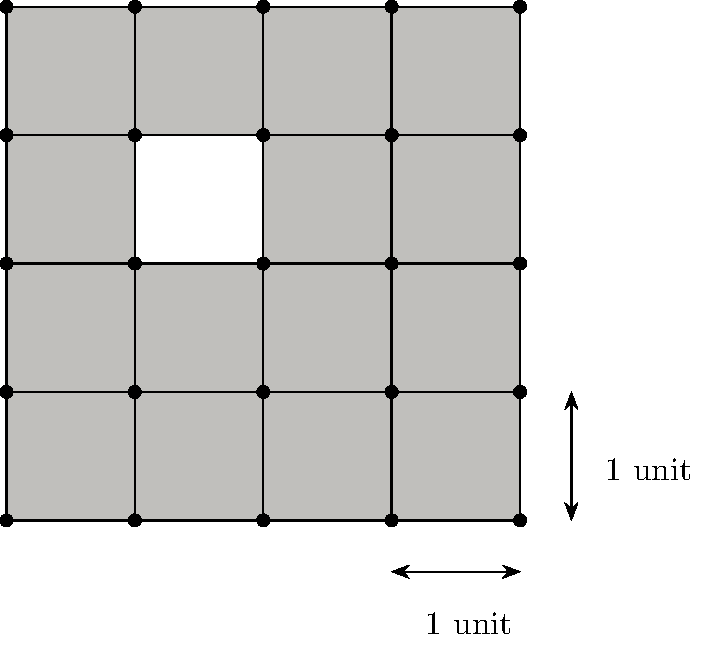
\includegraphics[width=0.5\linewidth]{fig/fig1.pdf}
	\end{figure}

	What is teh maximum number of squares without a "hole in the inrerior" that can be formed within the $4 \times 4$ grid using the unit squares as building blocks ?
             \begin{enumerate}
                   \item $15$
                   \item $20$
                   \item $21$
                   \item $26$
             \end{enumerate}
       \item An art gallery engages a security guard to ensure that the items displayed are protected. The diagram below represents the plan of the gallery where the boundary walls are opaque. The location the security guard posted is identified such that all the inner space (shaded region in the plan) of the gallery is within the line of sight of the security guard.

If the security guard does not move around the posted location and has a $360 \circ$ view, which one of the following correctly represents the set of ALL possible locations among the locations $P, Q, R$ and $S$, where the security guard can be posted to watch over the entire inner space of the gallery?
        \begin{figure}[ht!]
	    \centering
	    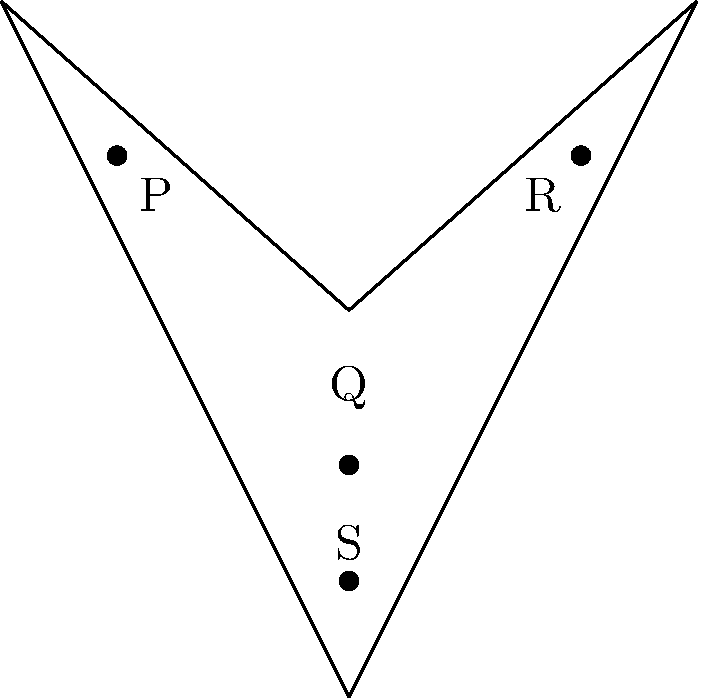
\includegraphics[width=0.3\linewidth]{fig/fig2.pdf}
	\end{figure}    \begin{enumerate}
        \item $P$ and $Q$
        \item $Q$
        \item $Q$ and $S$
        \item $R$ and $S$
    \end{enumerate}
	\item  Mosquitoes pose a threat to human health. Controlling mosquitoes using chemicals may have undesired consequences. In Florida, authorities have used genetically modified mosquitoes to control the overall mosquito population. It remains to be seen if this novel approach has unforeseen consequences.

Which one of the following is the correct logical inference based on the information in the above passage ?
        \begin{enumerate}
            \item Using chemicals to kill mosquitoes is better than using genetically modified mosquitoes because genetic engineering is dangerous
            \item Using genetically modified mosquitoes is better than using chemicals to kill mosquitoes because they do not have any side effects.
            \item Both using genetically modified mosquitoes and chemicals have undesired consequences and can be dangerous.
            \item Using chemicals to kill mosquitoes may have undesired consequences but it is not clear if using genetically modified mosquitoes has any negative consequence.
        \end{enumerate}
	\item Consider the following inequalities.\\ 
          \brak{i} $2x-1> 7$\\
          \brak{ii} $2x-9 <1$\\
          Which one of hte following expressions below satisfies the above two inequalities?
          \begin{enumerate}
              \item $x\leq -4$
              \item $-4<x \leq 4$
              \item $4<x<5$
              \item $x\geq 5$
          \end{enumerate}
	\item Four points $P\brak{0,1},Q\brak{0,-3},R\brak{-2,-1}$ and $S\brak{2,-1}$ represent teh vertices of a quadrilateral. What is the area enclosed by the quadrilateral?
    \begin{enumerate}
          \item $4$
          \item $4\sqrt{2}$
          \item $8$
          \item $8\sqrt{2}$
    \end{enumerate}
	\item In a class of five students $P,Q,R,S$ and $T$, only one student is known to have copied in the exam. The disciplinary committee has investigated the situation and recorded the statements from the students as given below.\\
    \textbf{statement of $P$}: $R$ has copied in the exam.\\
    \textbf{statement of $Q$}: $S$ has copied in the exam.\\
    \textbf{statement of $R$}: $P$ did not copy in the exam.\\
    \textbf{statement of $S$}: only one of us is telling the truth.\\
    \textbf{statement of $T$}: $R$ is telling the truth.\\
    The investigating team dad authentic information that $S$ never lies.\\
    Based on the information given above, teh person who has copied in the exam is 
    \begin{enumerate}
        \item $R$
        \item $P$
        \item $Q$
        \item $T$
    \end{enumerate}
         
	\item Consider the following square with the four corners and the center marked as $P$, $Q$, $R$, $S$, and $T$ respectively.\\
    Let $X$, $Y$, and $Z$ represent the following operations:\\
    $X$: Rotation of the square by $180$ degrees with respect to the $S$-$Q$ axis.\\
    $Y$: Rotation of the square by $180$ degrees with respect to the $P$-$R$ axis.\\
    $Z$: Rotation of the square by $90$ degrees clockwise with respect to the axis perpendicular, going into the screen and passing through the point $T$.\\
    Consider the following three distinct sequences of operations (which are applied in the left to right order):\\
    \brak{1} $XYZ$\\
    \brak{2} $XY$\\
    \brak{3} $ZZZZ$\\
    \begin{figure}[ht!]
	    \centering
	    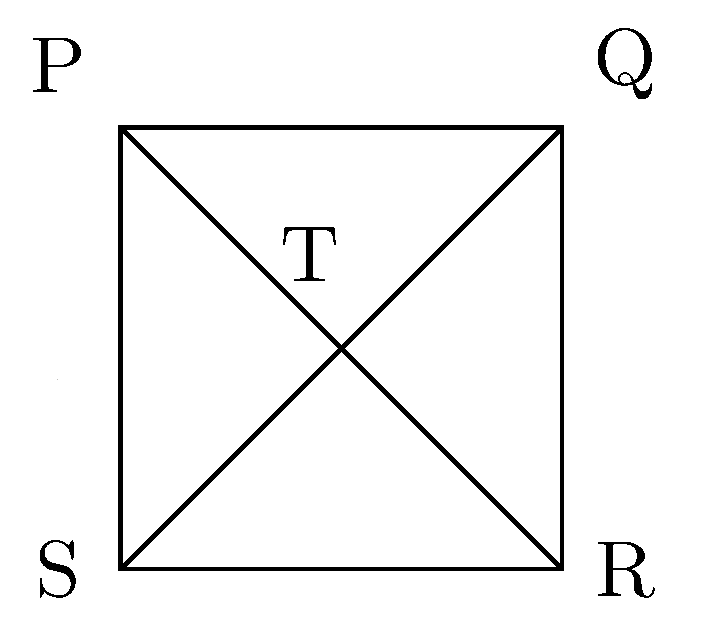
\includegraphics[width=0.3\linewidth]{fig/fig3.pdf}
	\end{figure}    Which one of the following statements is correct as per the information provided above?
    \begin{enumerate}
          \item The sequence of operations $\brak{1}$ and $\brak{2}$ are equivalent.
          \item The sequence of operations $\brak{1}$ and $\brak{3}$ are equivalent..
          \item The sequence of operations $\brak{2}$ and $\brak{3}$ are equivalent.
          \item The sequence of operations $\brak{1}$, $\brak{2}$, and $\brak{3} $ are equivalent.
    \end{enumerate}
    \textbf{Next $25$ carry ONE mark each}
    \item Let $\vec{M} $ be a $2\times 2$ real matix such that $\brak{\vec{I}+]vec{M}}^{-1}=\vec{I}-\alpha \vec{M}$, where $\alpha $ is a non-zero real number and $I$ is the $2\times 2$ identity matrix. If the trace of the matrix $\vec{M}$ is $3$, then the value of $\alpha$ is 
         \begin{enumerate}
               \item $\frac{3}{4}$
               \item $\frac{1}{3}$
               \item $\frac{1}{2}$
               \item $\frac{1}{4}$
         \end{enumerate}
    \item Let $\cbrak{X\brak{t}}_{t\geq 0}$ be a linear pure death process  with death rate $\mu_i =5i, i=0,1,\ldots ,N, N\geq 1$. Suppose that $p_i = P\brak{X\brak{t}=i}$. Then the system of forward Kolmogorov's equations is 
    \begin{enumerate}
        \item $\frac{dp_i\brak{t}}{dt} = 5\brak{i+1}p_{i+1}\brak{t} + 5i \, p_i\brak{t}$ 
and $\frac{dp_N\brak{t}}{dt} = 5N \, p_N\brak{t}$ for $i = 0, 1, 2, \ldots, N-1$ 
with initial conditions $p_i\brak{0} = 0$ for $i \neq N$, and $p_N\brak{0} = 1$.

        \item $\frac{dp_i\brak{t}}{dt} = 5\brak{i+1}p_{i+1}\brak{t} - 5i p_i\brak{t}$ 
\text{ and } 
$\frac{dp_N\brak{t}}{dt} = -5N p_N\brak{t}$ 
for $i = 0, 1, 2, \ldots, N-1$ with initial conditions $p_i\brak{0} = 0$ for $i \neq N$, and $p_N\brak{0} = 1$.

\item $\frac{dp_i\brak{t}}{dt} = 5\brak{i+1}p_{i+1}\brak{t} + 5i p_i\brak{t}$ 
\text{ and } 
$\frac{dp_N\brak{t}}{dt} = 5N p_N\brak{t}$ 
for $i = 0, 1, 2, \ldots, N-1$ with initial conditions $p_i\brak{0} = 1$ for $i \neq N$, and $p_N\brak{0} = 0$.

\item $\frac{dp_i\brak{t}}{dt} = 5\brak{i+1}p_{i+1}\brak{t} - 5i p_i\brak{t}$ 
\text{ and } 
$\frac{dp_N\brak{t}}{dt} = -5N p_N\brak{t}$ 
for $i = 0, 1, 2, \ldots, N-1$ with initial conditions $p_i\brak{0} = 1$ for $i \neq N$, and $p_N\brak{0} = 0$.

    \end{enumerate}
    \item Let $S^2$ be the variance of a random sample of size $n>1$ from a noramal population with an unknown mean $\mu$ and an unknown finite variance $\sigma ^2>0$. Consider the following statements:\\
    \brak{I} $S^2$ is an unbiased estimator of $\sigma ^2$ , and $S$ is an unbiased  estimator of $\sigma$\\
    \brak{II} $\brak{\frac{n-1}{n}}S^2$ is a maximum likelihood estimator of $\sigma ^2$, and $\sqrt{\frac{n-1}{n}}S$ is a maximum likelihood estimator of $\sigma$.\\
    Which of the above statements is/are true?
    \begin{enumerate}
        \item \brak{I} only 
        \item \brak{II} only 
        \item Both \brak{I} and \brak{II}
        \item Neither \brak{I} and \brak{II}
    \end{enumerate}
    
\end{enumerate}	
\end{document}


